\subsection{関手圏}\label{chap-7.1-functor-category}
	自然変換には恒等射によって定義される恒等自然変換と、射の合成によって定義される垂直変換を考えることができた。これまで様々な圏を考えてきたように、これらの自然変換を用いれば実際に圏を考えることができるようになる。
	\begin{define}[関手圏]\label{def-functor-category}
		二つの圏$\cat{C,D}$に対する\textbf{関手圏}$\funccat{C}{D}$を以下の要素で定義する。
		\begin{quote}
			\begin{mydescription}
				\item[対象] $\obj{\funccat{C}{D}}$を$\cat{C}$から$\cat{D}$への関手の全体とする。すなわち、$\cat{Cat}$における射集合によって$\obj{\funccat{C}{D}}=\arset{Cat}{\cat{C}}{\cat{D}}$と表せる。
				\item[射]任意の関手$\functor{F,G}{C}{D}$に対して、射集合$\arset{\funccat{C}{D}}{F}{G}$を関手$F,G$の間の自然変換全体の集合とする。
				\item[射の合成] 任意の関手$\functor{F,G,H}{C}{D}$の間の任意の自然変換$\nat{\alpha}{F}{G}$、$\nat{\beta}{G}{H}$を合成した自然変換を、自然変換の垂直合成によって$\beta\cdot\alpha$と定義する。
				\item[恒等射の存在]任意の関手$\functor{F}{C}{D}$に対して、恒等射となる自然変換を恒等自然変換によって$ID_F$と定義する。
				\item[結合律]任意の関手$\functor{F,G,H,I}{C}{D}$と自然変換$\nat{\alpha}{F}{G}$、$\nat{\beta}{G}{H}$、$\nat{\gamma}{H}{I}$に対して、\[(\gamma\cdot\beta)\cdot\alpha=\gamma\cdot(\beta\cdot\alpha)\]が成り立てば良い。
				自然変換の成分はただの射であるから圏$\cat{D}$の結合律より、圏$\cat{C}$の任意の対象$X$に対して

        \begin{align*}
          ((\gamma\cdot\beta)\cdot\alpha)_X&=(\gamma_X\circ\beta_X)\circ\alpha_X&\text{(自然変換の垂直合成の定義)}\\
          &=\gamma_X\circ(\beta_X\circ\alpha_X)&\text{(圏$\cat{D}$の結合律)}\\
          &=(\gamma\cdot(\beta\cdot\alpha))_X&\text{(自然変換の垂直合成の定義)}\\
        \end{align*}
        が成り立つ。よって二つの自然変換のすべての成分が一致するから$(\gamma\cdot\beta)\cdot\alpha=\gamma\cdot(\beta\cdot\alpha)$であり、結合律が成り立つ。
				\item[単位元律] 任意の関手$\functor{G}{C}{D}$に対応する恒等自然変換$ID_G$と、任意の関手$\functor{F,H}{C}{D}$、任意の自然変換$\nat{\alpha}{F}{G}$、$\nat{\beta}{G}{H}$に対して、
        \[ID_G\cdot\alpha=\alpha,\, \beta\cdot ID_G=\beta\]が成り立つことを示せば良い。
				結合律と同様に成分を考える。恒等自然変換の成分は恒等射であるから、圏$\cat{C}$の任意の対象$X$に対して
        \begin{align*}
          (ID_G\cdot\alpha)_X&=(ID_G)_X\circ\alpha_X&\text{(自然変換の垂直合成の定義)}\\
          &=id_{GX}\circ\alpha_X&\text{恒等自然変換の定義}\\
          &=\alpha_X&\text{圏$\cat{D}$の単位元律}
        \end{align*}
        $\beta$に対しても同様に示せる。よって$ID_G\cdot\alpha=\alpha,\, \beta\cdot ID_G=\beta$であり、単位元律が成り立つ。
			\end{mydescription}
		\end{quote}
	\end{define}
  まだ圏論的な操作からは関手圏を定義することはできないが、関手圏の対象の集合や射集合が定義できることは関手、自然変換が写像、射集合を用いて定義されていることから簡単に分かる。

  関手圏が圏であるということは、関手圏は$\cat{Cat}$の対象である。つまりある圏からある関手圏への関手を考えることができるようになる。その一例として定写像から対角写像を得たように、定関手を得る操作を関手と見なした対角関手を見ていこう。\\
  \begin{define}[対角関手]\label{def-diagonal-functor}
    圏$\cat{C}$から$\cat{D}$への定関手を与える対角関手$\functor{\varDelta}{D}{\funccat{C}{D}}$を以下のように定義する。
    \begin{quote}
			\begin{mydescription}
				\item[対象関数] 対象関数\[\mor{\varDelta}{\obj{D}}{\obj{\funccat{C}{D}}}\]
				を圏$\cat{D}$の任意の対象$D$と定関手$\functor{\varDelta D}{C}{D}$に対して定関数$\varDelta(D)=\varDelta D$と定義する。またここでの$\varDelta D$は射関数ではなく
				\item[射関数] 
        射関数は\[\mor{\varDelta}{\arset{C}{A}{B}}{\arset{\funccat{C}{D}}{\varDelta A}{\varDelta B}}\]となるように、$A$から$B$への射を、$A$の定関手から$B$の定関手への自然変換に写す写像になる。またこの自然変換を射$f$に対する定自然変換と呼ぶことにする。

        まずは任意の射$\mor{f}{A}{B}$に対する定自然変換$\nat{\varDelta f}{\varDelta A}{\varDelta B}$を先に定義する。
        圏$\cat{C}$の任意の対象$C$に対する$\varDelta f$の成分は\[\mor{(\varDelta f)_C}{\varDelta A(C)}{\varDelta B(C)}\]となるが、定関手の定義より、\[\mor{(\varDelta f)_C}{A}{B}\]と表せる。つまり、二つの定関手によって定自然変換の始域と終域がそれぞれ$A,B$に集約されているため成分を$(\varDelta f)_C=f$と定義できる。

        自然性については、\[(\varDelta f)_{C'}\circ\varDelta A(g)=f\circ id_A=id_B\circ f=\varDelta B(g)\circ(\varDelta f)_C\]と成り立ち、$\varDelta f$が自然変換であることが分かった。

        \begin{center}
          \begin{tikzpicture}[auto]
            \node (A) at (0, 1) {$C$};
            \node (B) at (2, 1) {$C'$};
            \node (FA') at (4, 2) {$\varDelta A(C)$};
            \node (FB') at (6, 2) {$\varDelta A(C')$};
            \node (GA') at (4, 0) {$\varDelta B(C)$};
            \node (GB') at (6, 0) {$\varDelta B(C')$};
      
            \node (FA) at (8, 2) {$A$};
            \node (FB) at (10, 2) {$A$};
            \node (GA) at (8, 0) {$B$};
            \node (GB) at (10, 0) {$B$};

            \node (e) at (7, 1) {$=$};
            \node (catc) at (1, 3.5) {$\cat{C}$};
            \node (catd) at (5, 3.5) {$\cat{D}$};
      
            \draw[->] (A) to node{$g$}(B);

            \draw[->] (FA) to node{$id_A$}(FB);
            \draw[->] (FA) to node[swap]{$f$}(GA);
            \draw[->] (FB) to node{$f$}(GB);
            \draw[->] (GA) to node{$id_B$}(GB);

            \draw[->] (FA') to node{$\varDelta A(g)$}(FB');
            \draw[->] (GA') to node{$\varDelta B(g)$}(GB');
            \draw[->] (FA') to node[swap]{$(\varDelta f)_C$}(GA');
            \draw[->] (FB') to node[swap]{$(\varDelta f)_C'$}(GB');
            \draw[->,bend left = 20] (catc) to node (funcf){$\varDelta A$}(catd);
            \draw[->,bend right = 20] (catc) to node (funcg)[swap]{$\varDelta B$}(catd);
            \draw[double,double equal sign distance,-implies,shorten >=5pt,shorten <=5pt] (funcf) -- node[label=right:$\varDelta f$] {} (funcg);
          \end{tikzpicture}
        \end{center}

        これによって、対角関手の射関数$\mor{\varDelta}{\arset{C}{A}{B}}{\arset{\funccat{C}{D}}{\varDelta A}{\varDelta B}}$を$\varDelta(f)=\varDelta f$と定義する。

				\item[恒等射の保存] 圏$\cat{D}$の任意の対象$D$に対して$\varDelta(id_D)=ID_{\varDelta D}$を示せば良い。また対角関手の終域は関手圏であるため、関手圏の恒等射である恒等自然変換に対応する。
        圏$\cat{C}$の任意の対象$C$の成分を見ると、
        \begin{align*}
          (\varDelta (id_D))_C &= id_D &\text{(射関数の定義)}\\
          (ID_{\varDelta D})_C &= id_{\varDelta D(C)}&\text{(恒等自然変換の定義)}\\
          &= id_D&\text{(定関手の定義)}
        \end{align*}
        よって任意の成分について\[(\varDelta (id_D))_C=id_D=(ID_{\varDelta D})_C\]が成り立つから$\varDelta(id_D)=ID_{\varDelta D}$となり、恒等射を保存する。

				\item[射の合成の保存] 圏$\cat{D}$の合成可能な二射$f,g$に対して、$\varDelta(g\circ f)=\varDelta g\circ \varDelta f$が成り立てばよい。同様に圏$\cat{C}$の任意の対象$C$に対する成分を見ると、
        \begin{align*}
          (\varDelta(g\circ f))_C&=g\circ f&\text{(射関数の定義)}\\
          (\varDelta g\cdot\varDelta f)_C &= (\varDelta g)_C\circ (\varDelta f)_C&\text{(自然変換の垂直合成の定義)}\\
          &=g\circ f&\text{(射関数の定義)}
        \end{align*}
        よって任意の成分について\[(\varDelta(g\circ f))_C=g\circ f=(\varDelta g)_C\circ (\varDelta f)_C\]が成り立つから$\varDelta(g\circ f)=\varDelta g\circ \varDelta f$となり、射の合成を保存する。
			\end{mydescription}
		\end{quote}
  \end{define}

  圏から関手圏への関手が違和感なく定義される事が分かったと思う。次は更に踏み込んで圏と関手圏の間の同型を示す。\\
  また圏の同型についても軽く触れておこう。
  \begin{define}[圏同型]\label{def-isomorphic-of-categories}
    $\cat{Cat}$において、圏$\cat{C,D}$が関手$\functor{I}{C}{D},\ \functor{I^{-1}}{D}{C}$によって同型、つまり$I\circ I^{-1}=Id_D,\ I^{-1}\circ I=Id_C$である時、圏同型と呼ぶことにする。またこの時関手$I,I^{-1}$を\textbf{同型関手}と呼ぶことにする。
  \end{define}
  一般の圏と同様に元の対応を見てみよう。同型の元の関係より、$\functor{C}{1}{C}$は$\cat{C}$の対象と同一視できるのだった。すなわちある対象$D$が存在して$C\sim D$となる。\\

  \begin{center}
    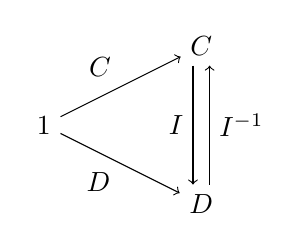
\begin{tikzpicture}[auto]
      \node (1) at (-2, 1) {$\cat{1}$};
      \node (a) at (0, 2) {$\cat{C}$};
      \node (b) at (0, 0) {$\cat{D}$};
      \draw[->] (1) to node{$C$}(a);
      \draw[->] (1) to node[swap]{$D$}(b);
      \draw[->,transform canvas={xshift=-3pt}] (a) to node[swap] {$I$}(b);
      \draw[->,transform canvas={xshift=3pt}] (b) to node[swap] {$I^{-1}$}(a);
    \end{tikzpicture}
  \end{center}
  関手の定義に乗っ取ると、関手$I\circ I^{-1}$の対象関数は合成関手の定義より、それぞれの対象関数\[\mor{I}{\obj{C}}{\obj{D}},\ \mor{I^{-1}}{\obj{D}}{\obj{C}}\]の合成\[\mor{I\circ I^{-1}}{\obj{D}}{\obj{D}}\]が対象関数になる。$I\circ I^{-1}=Id_\cat{D}$であるから、対象関数においても$I\circ I^{-1}=id_{\obj{D}}$が成り立つ。同様に$I^{-1}\circ I=id_{\obj{C}}$も成り立つから、$I,I^{-1}$の対象関数も$\cat{Set}$上の同型射となる。

  次に圏の射の対応関係を見ていこう。
  関手の定義に従って考えると、関手$I\circ I^{-1}$の射関数は、合成関手の定義よりそれぞれの射関数$\mor{I}{\arset{C}{A}{B}}{\arset{D}{IA}{IB}}$、$\mor{I^{-1}}{\arset{D}{A}{B}}{\arset{C}{I^{-1}A}{I^{-1}B}}$の合成射
  \[\mor{I\circ I^{-1}}{\arset{D}{A}{B}}{\arset{D}{A}{B}}\]が射関数となる。対象関数と同様にこれも同型射になるから、射$\mor{f}{C}{C'}$に対して$Ff=g,\ C\sim D, C'\sim D'$とすると同型$\arset{C}{C}{C'}\cong\arset{D}{D}{D'}$によって$f\sim g$と表記できる。
  \begin{center}
    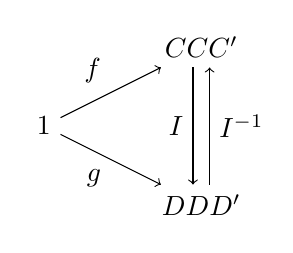
\begin{tikzpicture}[auto]
      \node (1) at (-2, 1) {$1$};
      \node (a) at (0, 2) {$\arset{C}{C}{C'}$};
      \node (b) at (0, 0) {$\arset{D}{D}{D'}$};
      \draw[->] (1) to node{$f$}(a);
      \draw[->] (1) to node[swap]{$g$}(b);
      \draw[->,transform canvas={xshift=-3pt}] (a) to node[swap] {$I$}(b);
      \draw[->,transform canvas={xshift=3pt}] (b) to node[swap] {$I^{-1}$}(a);
    \end{tikzpicture}
  \end{center}  
  \begin{prop}[圏の元]\label{prop-elements-of-category}
    一点離散圏$\cat{1}$、任意の圏$\cat{C}$に対して$\cat{C}\cong\funccat{1}{C}$
  \end{prop}
  \begin{proof}
    集合の圏における同型$A\cong\arset{Set}{1}{A}$と同様の手法で証明する。
    すなわち、対角関手$\functor{\varDelta}{C}{\funccat{1}{C}}$が同型射となる関手であることを示す。\\
    また定写像と同様に$\funccat{1}{C}$の対象である任意の関手は明らかに定関手である。なぜなら一点離散圏$\cat{1}$はただ一つの対象と射のみを持ち、それらは必ず圏$\cat{C}$のただ一つの対象とその恒等射に写されるため、定関手の定義を満たす。\\
    関手$\functor{\varDelta^{-1}}{C^1}{C}$を
    \begin{quote}
			\begin{mydescription}
				\item[対象関数]対象関数\[\mor{\varDelta^{-1}}{\obj{C^1}}{\obj{C}}\]を圏$\funccat{C}{1}$の任意の対象$\varDelta A$に対して$\varDelta^{-1}(\varDelta A)=\varDelta A(*)=A$と定義する。\\
        この対象関数の全域性は先ほど示した$\funccat{C}{1}$の性質によるものである。
				\item[射関数]射関数\[\mor{\varDelta^{-1}}{\arset{\funccat{1}{C}}{\varDelta A}{\varDelta B}}{\arset{C}{A}{B}}\]を任意の定自然変換$\nat{\varDelta f}{\varDelta A}{\varDelta B}$に対して$\varDelta^{-1}(\varDelta f) = (\varDelta f)_*=f$と定義する。
				\item[恒等射の保存]任意の対象$A$に対して$\varDelta^{-1}(ID_{\varDelta_A})=id_{\varDelta^{-1}(\varDelta A)}$を示せばよい。これは対角関手の恒等射の保存から簡単に示せる。
				\begin{align*}
          \varDelta^{-1}(ID_{\varDelta A})&=\varDelta^{-1}(\varDelta id_A)&\text{(対角関手の恒等射の保存)}\\
          &=id_A&\text{(射関数の定義)}\\
          &=id_{\varDelta^{-1}(\varDelta A)}&\text{(対象関数の定義)}
        \end{align*}
        よって成り立つ。
				\item[射の合成の保存]任意の合成可能な二射$f,g$に対して、$\varDelta^{-1}(\varDelta g\cdot\varDelta f)=\varDelta^{-1}(\varDelta g)\circ\varDelta^{-1}(\varDelta f)$が成り立つことを示せばよい。同様に対角関手の射の合成の保存から簡単に示せる。
				\begin{align*}
          \varDelta^{-1}(\varDelta g\cdot\varDelta f)&=\varDelta^{-1}(\varDelta(g\circ f))&\text{(対角関手の射の合成の保存)}\\
          &=g\circ f&\text{(射関数の定義)}\\
          &=\varDelta^{-1}(\varDelta g)\circ\varDelta^{-1}(\varDelta f)&\text{(射関数の定義)}
        \end{align*}
			\end{mydescription}
		\end{quote}
    対象関数$\varDelta,\ \varDelta^{-1}$において、圏$\cat{C}$の任意の対象$A$に対して
    \begin{align*}
      A&=\varDelta^{-1}(\varDelta A)\\
      &=(\varDelta^{-1}\circ\varDelta)(A)
    \end{align*}
    であるから、$\varDelta^{-1}\circ\varDelta=id_\obj{C}$が成り立つ。\\
    圏$\funccat{C}{1}$の任意の対象$F$を考えるが、$\funccat{C}{1}$の任意の対象は定関手であるため、任意の定関手$\varDelta A$を考えればよい。よって
    \begin{align*}
      F&=\varDelta A\\
      &=\varDelta((\varDelta^{-1}\circ\varDelta)(A))\\
      &=(\varDelta\circ \varDelta^{-1})(\varDelta A)\\
      &=(\varDelta\circ \varDelta^{-1})(F)
    \end{align*}
    よって、$\varDelta\circ\varDelta^{-1}=id_\obj{C^1}$が成り立つ。\\
    同様の議論が射関数でも成り立つから、射関数、対象関数の等式により$\varDelta^{-1}\circ\varDelta=Id_\cat{C},\ \varDelta\circ\varDelta^{-1}=Id_\funccat{C}{1}$となり、$\cat{C}\cong\funccat{1}{C}$が成り立つ。
  \end{proof}
  圏$\cat{C}$の対象は関手$\functor{\varDelta A}{1}{C}$で表現でき、射は自然変換$\nat{\varDelta f}{\varDelta A}{\varDelta B}$で表現できることになるが、これによって圏の対象や射といった内部の構造に言及せずとも圏に関する議論を行うことができるようになった。\\
  また以降の議論で紛らわしくない場合、$\funccat{1}{C}$の対象$\varDelta A$を$A$、射$\varDelta f$を$f$と表記することにする。